% !TeX encoding = UTF-8
% !TeX spellcheck = en_US
% !TeX root = ../../../main.tex

\section{The framework}
\label{sec:framework}

The following section describes the framework which was developed during this thesis and how it could be used and configured. The framework was developed in two iterations. The first iteration was merely used during the initial experiments and resulted in a collection of \MATLAB scripts, barely useful for reuse but brought some insights into the possibilities of \MATLAB and for the next version of the framework. The second iteration was developed with having a future reuse and extendability in mind.

\subsection{First version}

\begin{wrapfigure}{r}{0.4\textwidth}
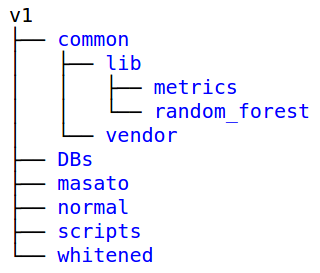
\includegraphics[width=\textwidth]{content/pictures/v1_dirs.png}
\caption{Framework v1 Directory layout}
\label{fig:framework_v1_dirs}
\end{wrapfigure}

The first version of the framework has its primary focus on the experiments involving different feature algorithms and the general investigation of the basic codebook performance. The main directory for the implemented \MATLAB scripts is the \textit{common} folder. It contains 16 files which are responsible for the extraction of features, clustering with k-Means and \ac{GMM}, generation of codebooks and visualization of the codebook comparisons. These scripts share and use in total 57 functions which resides inside the \textit{common/lib} folder to accomplish their work. As the experiments in this stage were done with \ac{HOG} and \ac{WHOG} in parallel, the folders \textit{normal} and \textit{whitened} respectively contain independent settings and scripts which require a different handling based on the used feature backend. The \textit{scripts} folder contain some shell and utility scripts for setting up the environment and launching the different experiments. The \ac{VOC2011} dataset resides in the \textit{DBs} folder and the \textit{masato} folder contains some helper functions provided to me by Masato Takami. Beside of these helper functions, all other functions or libraries not written by myself are located in \textit{common/vendor}. This includes the ExemplarSVM \cite{Malisiewicz2011}, yael \cite{yael} and flann \cite{muja_flann_2009} libraries.

Depending on the chosen feature backend a folder with an optional tag (for example \textit{data\_boxed-approach} or \textit{data\_svm}) is created inside the \textit{normal} or \textit{whitened} folder by the setup scripts. This data folder is afterwards used throughout all scripts and functions as a target for the experiment results and within a \textit{cache} subfolder for caching the results. The cached data includes

\begin{itemize}
\item Features per image as
    \begin{itemize}
    \item boxed $\Rightarrow$ only the first bounding box for the current class is stored
    \item inverted boxed sliding $\Rightarrow$ everything except the bounding boxes for the current class in a sliding window manner. Used for the negative set during the \ac{SVM} training.
    \item custom $\Rightarrow$ used for the first implementation of integral images, typically the complete image
    \end{itemize}
\item Codebooks, organized by
    \begin{itemize}
    \item \dots their number of dimensions.
    \item \dots the number of parts per window.
    \item \dots the feature type as for the cached features.
    \end{itemize}
\item \acp{SVM}, organized like the codebooks with an additional separation if trained with
    \begin{itemize}
    \item \dots k-Means clusters.
    \item \dots fisher vectors.
    \end{itemize}
\end{itemize}

During the development process several utility applications were created with the python\footnote{\url{https://www.python.org}} programming language. The two main applications are \ac{GUI} based programs to work with a list of PASCAL images and group them in up to four different lists or remove some of the images from a list. The first application was written because it was required during the experiments to create multiple lists of bicycles, grouped by their orientation. As the image lists contained a high amount of images and the verification of which image is meant by a given image id was a time consuming task, the second application was written to simplify the removal of images from a given list. Both applications can be found in the git repository at \url{https://github.com/bluec0re/pascal-utils}\footnote{Revision at the time of writting: 7a4be4c941a03bc2810dd2fbbec3f336ff38fdc3}.

\subsection{Second version}

After the first experiments with the feature algorithms, codebook dimensions and \ac{SVM} usage were done, the second version of the framework was developed.
%TODO beschreibung des frameworks

%\begin{table}
\begin{longtable}{%
|%
p{0.2\textwidth}%
|%
>{\raggedright\arraybackslash}%
p{0.135\textwidth}%
|%
>{\raggedright\arraybackslash}%
p{0.135\textwidth}%
|%
>{\raggedright\arraybackslash}%
p{0.4\textwidth}%
|%
}
\hline \textbf{Parameter} & \textbf{Possible values} & \textbf{Default} & \textbf{Description} \\ 
\hline
\hline class & A PASCAL class & bicycle & Specifies the class to restrict the bounding boxes to \\ 
\hline parts & $x \in \mathbb{N} \textbackslash 0$ & 4 & Number of parts per window \\ 
\hline clusters & $x \in \mathbb{N} \textbackslash 0$ & 1000 & Number of k-Means clusters to use \\ 
\hline integrals\allowbreak\_scale\allowbreak\_factor & $x \in \mathbb{R}, 0 < x \le 1$ & 1 & Specifies the percentage to which a integral image should be downsampled to \\ 
\hline stream\allowbreak\_max & $x \in \mathbb{N} \textbackslash 0$ & 100 & Maximum amount of images used from a PASCAL stream \\ 
\hline stream\allowbreak\_name & Any string & query & Name of the PASCAL stream to read images from \\ 
\hline codebook\allowbreak\_type & double, single & double & Internal datatype of the codebooks \\ 
\hline codebook\allowbreak\_scales\allowbreak\_count & $x \in \mathbb{N} \textbackslash 0$ & 3 & Amount of scale ranges in which integral images will be split into \\ 
\hline nonmax\allowbreak\_type\allowbreak\_min & true, false & true & Specifies if $\frac{\text{area}(A \cap B)}{\min(\text{area}(A), \text{area}(B))}$ or $\frac{\text{area}(A \cap B)}{\text{area}(A \cup B)}$ should be used for a non-maximum suppression \\ 
\hline use\allowbreak\_calibration & true, false & true & If true, a score calibration based on the query image is performed \\ 
\hline features\allowbreak\_per\allowbreak\_roi & $x \in \mathbb{R}, 0 < x$ & 2 & Amount of feature patches which have to exist per window axis \\ 
\hline query\allowbreak\_from\allowbreak\_integral & true, false & false & If true, the query codebooks will be retrieved from the image database instead of extracted from the query image \\ 
\hline default\allowbreak\_query\allowbreak\_file & An image id & 2008\allowbreak\_004363 & Used to automate the experiments instead of asking interactively for a query image \\ 
\hline default\allowbreak\_bounding\allowbreak\_box & [x, y, width, height] & Extracted from the PASCAL dataset & The bounding box of the query image part \\ 
\hline use\allowbreak\_libsvm\allowbreak\_classification & true, false & true & If true, the \verb|svmpredict| function is used to classify the database codebooks. Otherwise a custom implementation is used \\ 
\hline expand\allowbreak\_bboxes & true, false & true & Expands the bounding boxes by $\frac{1}{2}$ of the average feature patch size \\ 
\hline naiive\allowbreak\_integral\allowbreak\_backend & true, false & true & Specifies to use full integral images without any memory optimization techniques \\ 
\hline window\allowbreak\_margin & $x \in \mathbb{N} \textbackslash 0$ & 10 & Amount of pixels each window is shifted during the sliding window generation  \\ 
\hline max\allowbreak\_window\allowbreak\_scales & $x \in \mathbb{N} \textbackslash 0$ & 10 & Maximum amount of times a scaling is performed during the sliding window generation \\ 
\hline min\allowbreak\_window\allowbreak\_size & $x \in \mathbb{R}, 0 < x \le 1$ & 0.5 & Required percentage of a window area which has to be placed over an image (windows are getting clipped at the image boundaries)\\ 
\hline use\allowbreak\_kdtree & true, false & false & Enables the kd-Tree storage backend \\ 
\hline integral\allowbreak\_backend\allowbreak\_overwrite & true, false & false & Enables the integral matrix reconstruction via overwriting the bottom right values \\ 
\hline integral\allowbreak\_backend\allowbreak\_sum & true, false & false & Enables the integral matrix reconstruction via summing up the bottom right values \\ 
\hline integral\allowbreak\_backend\allowbreak\_matlab\allowbreak\_sparse & true, false & false & Enables the \MATLAB sparse storage backend \\ 
\hline precalced\allowbreak\_windows & true, false & false & Disables integral images and precalculates codebooks in a sliding window manner \\ 
\hline 
\caption{Configuration parameters for the part retrieval framework}
\label{tab:configuration_framework}
\end{longtable}
%\end{table}


\subsection{A modular approach}